\documentclass[a4paper,14pt]{article} % тип документа

\usepackage[T2A]{fontenc}			% кодировка
\usepackage[utf8]{inputenc}			% кодировка исходного текста
\usepackage[english,russian]{babel}	% локализация и переносы

\usepackage{extsizes} % Возможность сделать 14-й шрифт
\usepackage{geometry} % Простой способ задавать поля
\geometry{top=25mm}
\geometry{bottom=35mm}
\geometry{left=30mm}
\geometry{right=20mm}

% Математика
\usepackage{amsmath,amsfonts,amssymb,amsthm,mathtools} 
\usepackage{wasysym}
\usepackage{dsfont}
\usepackage{mathrsfs}
\usepackage{upgreek}

\usepackage{natbib}
\usepackage{graphicx}
\usepackage{indentfirst}

\begin{document}
	
	\section*{Билет номер 3}
	
	\subsection*{Частные производные функции нескольких переменных}  
	
	\textbf{Определение.} $f$ определена $\mathscr{U}(a) \subset \mathds{E}^m$. Если существует и конечен $\lim\limits_{\Delta{x_k}\to 0} \frac{\Delta_k f(a, \Delta{x_k})}{\Delta{x_k}}=b \in R$, то этот предел называется частной производной функции $w = f(x)$ в точке а по аргументу $x_k$.\\
	
	\textbf{Обозначение.}  $\frac{\partial f}{\partial x_k}(a)$ или $f'_{x_k}$
	\[\Delta_k f(a, \Delta{x_k}) = f(a_1, \ldots, a_{k-1}, a_k + \Delta x_k, a_{k+1}, \ldots, a_m) - f(a_1, \ldots, a_m)\] 
	\begin{center}
	(Только на месте k-ого аргумента есть приращение).\\
	\end{center}

	\textbf{Замечания.}
	 
	1. При вычислении  $\frac{\partial f}{\partial x_k}(x)$ вычисляется как для функций одной переменной $x_k$ при фиксированных остальных переменных (остальные переменные -- постоянные).\\
	
	2. $\left[\exists \frac{\partial f}{\partial x_j}(a), j = 1, \ldots, m\right] \not\Rightarrow [f$ непрерывна в точке а$]$ \\
	
	\textbf{Контрпример.}
	
	\begin{equation*}
		\omega = f(x, y) = 
		\begin{cases}
			\frac{2xy}{x^2 + y^2}, & x^2 + y^2 \not=0,\\
			0, & x^2 + y^2 = 0
		\end{cases}
	\end{equation*}
	\[\frac{\partial f}{\partial x}(0,0) = \lim_{x\to 0} \frac{f(x, 0) - f(0, 0)}{x} = 0\]
	\[\frac{\partial f}{\partial y}(0,0) = \lim_{y\to 0} \frac{f(0, y) - f(0, 0)}{y} = 0\]
	Однако, $f$ не является непрерывной в точке (0, 0), т.к. в этой точке у нее не существует $\lim\limits_{(x, y) \to (0, 0)} f(x, y)$.\\
	
	3. Определение частной произвоной функции $w = f(x)$ дано для внутренней точки множества определения функции. Оно не пригодно для граничной предельной точки множетсва, поскольку в граничной точке не всегда можно определить частное приращение. Поэтому частная производная в граничной предельной точке множества определения функции находиться как предел частной производной по множеству.
	
	Точка $a \in X$ -- предельная граничная точка. 
	\begin{figure}[h!]
		\centering
		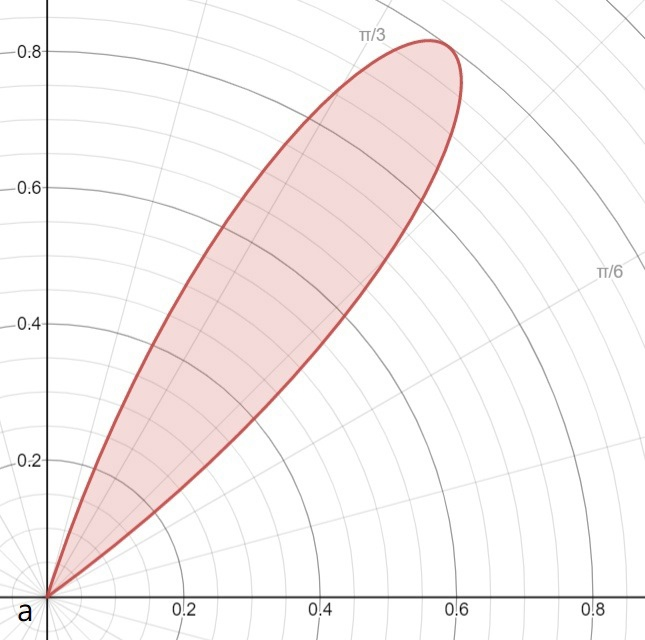
\includegraphics[scale=0.5]{Primer_1.jpg}
		\label{fig:universe}
	\end{figure}
	\[\frac{\partial f}{\partial x}(a) = \lim{_{(x, y)\to (a_1, a_2)}}_{(x, y) \in X} \frac{\partial f} {\partial x}(x, y)\]
	\[\frac{\partial f}{\partial y}(a) = \lim{_{(x, y)\to (a_1, a_2)}}_{(x, y) \in X} \frac{\partial f} {\partial y}(x, y)\]
	\subsection*{Дифференцируемость функции в точке}
	
	Некоторые замечания, которые нужны для определения дифференцируемости функции в точке:\\
	
	Рассмотрим $w = f(x)$, она определена в $\mathscr{U}(a), a = (a_1, \ldots,a_m), \Delta x = (\Delta x_1, \ldots, \Delta x_m): a + \Delta x = (a_1 + \Delta x_1, \ldots , a_m + \Delta x_m) \in \mathscr{U}(a)$\\
	
	Рассмотрим $\rho = \sqrt{(\Delta x_1)^2 + \ldots + (\Delta x_m)^2}$,  $\rho \to 0 \Leftrightarrow \Delta x \to \bar0$, где $\bar0 = (0, 0\ldots, 0_m)$.\\
	
	$\Delta f(a, \Delta x) = f(a + \Delta x) - f(a)$ -- Полное приращение функции в точке а, соответствующее приращению аргументов $\Delta x = (\Delta x_1, \ldots, \Delta x_m)$.\\
	
	\textbf{Определение.} Функция $f$ называется дифференцируемой в точке а, если 
	
	\textbf{Условие 1:}
	\[\Delta f(a, \Delta x) = A_1 \Delta x_1 + \ldots + A_m \Delta x_m + \alpha_1(\Delta x) \Delta x_1 + \ldots + \alpha_m (\Delta x)\Delta x_m\] 
	где $A_j$ -- постоянные, $j = 1,\ldots,m$, не зависят от $\Delta x$, $\alpha_j = \alpha_j(\Delta x)$ -- б.м. функции при $\Delta x \to 0$; $\alpha_j = 0$ при $\bar{\Delta x} = \bar0$.\\
	
	\textbf{Условие 2:}
	 \[\Delta f(a, \Delta x) = A_1 \Delta x_1 + \ldots + A_m \Delta x_m + o(\rho), \rho\to 0\]  
	 \begin{center}
	 (По сути $\rho$ -- расстояние от точки $\Delta x$ до $\bar0$).
	 \end{center}
	
	\textbf{Предложение.} Условия 1 и 2 определения дифференцируемости функции в точке эквиваленты.
	
	\textit{Доказательство.}\\
	1 $\Rightarrow$ 2\\
	Покажем, что $\alpha_1(\Delta x)\Delta x_1 + \ldots + \alpha_m(\Delta x)\Delta x_m = o(\rho), \rho \rightarrow 0, \rho \not= 0$.
	
	Заметим, что \[|\frac{x_j}{\rho}| \leq 1, \rho = \sqrt{(\Delta x_1)^2 + \ldots + (\Delta x_m)^2}\]
	\[|\alpha_1\Delta x_1 + \ldots \alpha_m\Delta x_m| \leq \rho(|\alpha_1|\frac{|\Delta x_1|}{\rho} + \ldots + |\alpha_m|\frac{|\Delta x_m|}{\rho}) \leq \rho(|\alpha_1| + \ldots + |\alpha_m|)\]
	
	В силу того, что $\rho \to 0 \Leftrightarrow \Delta x \to \bar0$, $\rho(|\alpha_1| + \ldots + |\alpha_m|)$ также стремиться к нулю, как конечная сумма б.м. функций.\\
	Значит, $\rho(|\alpha_1| + \ldots + |\alpha_m|) = o(\rho)$. Показали, что это выражение действительно есть б.м. функция.\\
	2 $\Leftarrow$ 1 
	
	\[o(\rho) = \frac{\rho^2}{\rho} \frac{o(\rho)}{\rho} = \frac{(\Delta x_1)^2 + \ldots + (\Delta x_m)^2}{\rho} \frac{o(\rho)}{\rho}\]
	\[o(\rho) = (\frac{\Delta x_1}{\rho}\frac{o(\rho)}{\rho})\Delta x_1 + \ldots + (\frac{\Delta x_m}{\rho}\frac{o(\rho)}{\rho})\Delta x_m \]
	Понятно, что $\alpha_j = \frac{\Delta x_j}{\rho}\frac{o(\rho)}{\rho}$, но $\frac {\Delta x_j}{\rho}$ величина ограниченная, а $\frac {o(\rho)}{\rho} \to 0, \rho \to 0 \Rightarrow $ при $\Delta x \to \bar 0$.
	$\alpha_j = 0, j = 1, \ldots, m$, только при $\Delta x = \bar0$.
	
	\textit{Доказано.}
	
	
	 \subsection*{Достаточные условия дифференцируемости функции в точке}
	 
	 \textbf{Теорема 2.} Пусть $w = f(x)$ определена в $\mathscr{U}(a) \subset \mathds{E}^m$
	 и в этой окрестности существуют $\frac{\partial f}{\partial x_j}, j = 1, \ldots, m$. 
	 Если  $\frac{\partial f}{\partial x_j}, j = 1, \ldots, m$ непрерывны в точке а, то функция f дифференцируема в точке а.\\
	 
	 \textit{Докательство.}\\
	 Проведем доказательство для $m = 2, w = f(x, y), a = (a_1, a_2)$. \\
	 Рассмотрим точку $(a_1 + \Delta x, a_2 + \Delta y) \in \mathscr{U}(a)$.\\\\
	 Рассмотрим 
	 \[\Delta f(a, (\Delta x, \Delta y)) = f(a_1 + \Delta x, a_2 + \Delta y) - f(a_1, a_2)\]
	 \begin{multline*}
	 \Delta f(a, (\Delta x, \Delta y)) = f(a_1 + \Delta x, a_2 + \Delta y) - \\
	 - f(a_1, a_2 + \Delta y) + f(a_1, a_2 + \Delta y) - f(a_1, a_2)
	 \end{multline*}
	 Введем функцию $\varphi(x) = f(x, a_2 + \Delta y)$ и $\psi(y) = f(a_1, y)$
	 \begin{multline*}
	 \Delta f(a, (\Delta x, \Delta y)) = \Delta\varphi(a_1, \Delta x) + \Delta\psi(a_2, \Delta y) = \\
	 = \varphi(a_1 + \Delta x) - \varphi(a_1) + \psi(a_2 + \Delta y) - \psi(a_2)
	 \end{multline*}
	 По теореме Лагранжа $\exists 0 < \theta_1 < 1$ и $\exists 0 < \theta_2 < 1:$
	 \[f(a_1 + \Delta x, a_2 + \Delta y) - f(a_1, a_2 + \Delta y) = f'_x(a_1 + \theta_1 \Delta x, a_2 + \Delta y)\Delta x\]
	 \[f(a_1, a_2 + \Delta y) - f(a_1, a_2) = f'_y(a_1, a_2 + \theta_2 \Delta y)\Delta y\]
	 \[f'_x(a_1 + \theta_1\Delta x, a_2 + \Delta y) = f'_x(a_1, a_2) + \alpha_1(\Delta x, \Delta y); \alpha_1 \to 0, (\Delta x, \Delta y) \to (0, 0)\]
	  \[f'_y(a_1, a_2 + \theta_2 \Delta y) = f'_y(a_1, a_2) + \alpha_2(\Delta x, \Delta y); \alpha_2 \to 0,  (\Delta x, \Delta y) \to (0, 0)\]
	  \[\Delta f(a, (\Delta x, \Delta y)) = f'_x(a)\Delta x +f'_y(a)\Delta y + \alpha_1\Delta x + \alpha_2 \Delta y\]. Это в точности определение дифференцируемости функции $f$ в точке $а$.
	  
	  \textit{Доказано.}	  \\
	  
	 \textbf{Примеры.} (Доказательство дифференцируемости ф-ции в точке)\\
	 $w = f(x, y), \bar0 = (0,0), \rho = \sqrt{x^2 + y^2 }$\\ 
	 $f(x, y) - f(0, 0)= \frac{\partial f}{\partial x}(0, 0)\Delta x + \frac{\partial f}{\partial y}(0, 0)\Delta y + o(\rho), \rho \to 0$.\\
	 
	 \textbf{Пример 1.} $f(x, y) = y^2 \sin x$\\
	 Заметим, что $f(x, 0) = f(0, y) = f(0, 0) = 0$\\
	 Из определения частной производной: $\frac{\partial f}{\partial x}(0,0) = \lim\limits_{x\to0} \frac {f(x, 0) - f(0, 0)} {x} = 0$.\\
	  $\frac{\partial f}{\partial y}(0,0) = \lim\limits_{y\to0} \frac {f(0, y) - f(0, 0)} {y} = 0$.\\
	 Частные производные 0, значит надо показать, что $f(x, y) = o(\rho), \rho \to 0$.
	 Надо показать, что $F(x, y) = \frac{f(x, y)}{\sqrt{x^2 + y^2}} \to 0$, при $(x, y) \to (0, 0)$.\\
	 $|F(x, y)| = |\frac{y^2 \sin x}{\sqrt{x^2 + y^2}}| \leq \frac{y^2}{\sqrt{x^2 + y^2}} \leq (|y| \leq \sqrt{x^2 + y^2}) \leq \frac{\sqrt{x^2 + y^2}^2}{\sqrt{x^2 + y^2}} = \sqrt{x^2 + y^2} \leq \delta = \upvarepsilon$\\
	 $[\forall\upvarepsilon > 0  \exists\delta = \delta(\upvarepsilon) = \upvarepsilon: \forall(x, y): 0 < \rho = \sqrt{x^2 + y^2} < \delta \mapsto |F(x, y)| < \upvarepsilon] \stackrel{def}{=} [\lim\limits_{(x, y) \to (0, 0)} F(x, y) = 0] \Leftrightarrow [f(x, y) = o(\rho), \rho \to 0]$.\\
	 
	 \textbf{Пример 2.} $f(x, y) = \sqrt{|xy|}, \bar0 = (0, 0)$\\
	 $f(x, 0) = f(0, y) = f(0, 0) = 0 \Rightarrow \frac{\partial f}{\partial x}(0, 0) = \frac{\partial f}{\partial y}(0, 0) = 0$\\
	 $F(x, y) = \frac{\sqrt{|xy|}}{\sqrt{x^2 + y^2}}$ Перейдем к полярным координатам: $x = \rho \cos \varphi, y = \rho \sin \varphi$, $F(x, y) = \sqrt{|\cos \varphi\sin \varphi|}$\\
	 $\varphi = \frac{\pi}{2} \Rightarrow F(\rho, \varphi) = 0$\\
	 $\varphi = \frac{\pi}{4} \Rightarrow F(\rho, \varphi) = \frac{1}{\sqrt{2}} \not= 0$\\
	 Значит, f не является дифференцируемой в точке (0, 0).\\
	
	 \textbf{Пример 3.(Очень важный для понимания теории)} 
	 \begin{equation*}
	 	f(x, y) = 
	 	\begin{cases}
	 		(x^2 + y^2)\sin{\frac{1}{\sqrt{x^2 + y^2}}}, & x^2 + y^2 \not=0,\\
	 		0, & x^2 + y^2 = 0
	 	\end{cases}
	 \end{equation*}\\
 	 $f(x, 0) = x^2\sin{\frac{1}{|x|}}, x \not =0$\\
	 $f(0, y) = y^2\sin{\frac{1}{|y|}}, y \not =0$\\ 	
	 $f(0,0) = 0$\\
	 $\frac{\partial f}{\partial x}(0, 0) = \lim\limits_{x \to 0} = \frac{f(x, 0) - f(0, 0))}{x} = \lim\limits_{x \to 0} x\sin{\frac{1}{|x|}} = 0$ \\
	 $\frac{\partial f}{\partial y}(0, 0) = \lim\limits_{y \to 0} = \frac{f(0, y) - f(0, 0))}{y} = \lim\limits_{y \to 0} y\sin{\frac{1}{|y|}} = 0$\\\\
	 Теперь докажем, что эта функция дифференцируема в (0, 0)\\
	 Введем функцию \[F(x, y) = \frac{f(x, y)}{\sqrt{x^2 + y^2}} = \sqrt{x^2 + y^2}\sin{\frac{1}{\sqrt{x^2 + y^2}}}\]\\
	 $|F(x, y)| \leq \sqrt{x^2 + y^2} < \delta = \upvarepsilon$
	 \begin{multline*}
	 [\forall\upvarepsilon > 0  \exists\delta = \delta(\upvarepsilon) = \upvarepsilon: \forall(x, y): 0 < \rho = \sqrt{x^2 + y^2} < \delta \mapsto |F(x, y)| < \upvarepsilon] \stackrel{def}{=} \\
	 [\lim\limits_{(x, y) \to (0, 0)} F(x, y) = 0] \Leftrightarrow [f(x, y) = o(\rho), \rho \to 0].
	 \end{multline*}
	 $\Rightarrow f$ дифференцируема в (0, 0).\\
	 
	 Посмотрим на частные производные этой функции по x и y вне точки (0, 0):\\

	 \[\frac{\partial f}{\partial x}(x, y) = 2x\sin{\frac{1}{\sqrt{x^2+y^2}}} -\frac{x^2+y^2}{(\sqrt{x^2+y^2})^3} \cos{\frac{1}{\sqrt{x^2+y^2}}}\]

	 $\lim\limits_{(x, y) \to (0, 0)} \frac{\partial f}{\partial x}(x, y)$ не существует $\Rightarrow f'_x$ не является непрерывной в (0, 0).\\
	 Пример показывает, что непрерывность частных производных в точке не является необходимым условием дифференцируемости функции.\\
	 
	 \textbf{Замечание.} Непрерывность частных производных функции f в точке не является необходимым условием дифференцируемости функции в точке. Это условие достаточно(Теорема 2).\\
	 
	 \subsection*{Дифференцируемость сложной функции}
	 
	 Рассматриваем функции $x_j = \varphi_j(t)$ в окрестности точки $t^0 = (t_1^0, \ldots, t_k^0)\in \mathds{E}^k, j = 1, \ldots, m$.\\
	 Рассматриваем функцию $w = f(x),$которая определена в окрестности точки $a = (a_1, \ldots, a_m)$, причем $a_j = \varphi_j(t^0), j = 1, \ldots, m$.\\
	 $F(t) = f(\varphi_1(t), \ldots, \varphi_m(t))$ -- суперпозиция функций f и функций $\varphi_1(t) \ldots$ (сложная функция)\\
	 
	 \textbf{Теорема 3. [О дифференцируемости сложной функции]}
	 
	 Пусть функции $\varphi_j, j = 1, \ldots, m$ дифференцируемы в точке $t^0$, функция f дифференцируема в точке а, причем $a_j = \varphi_j(t^0), j = 1, \ldots,m$. Тогда $F(t) = f(\varphi_1(t), \ldots, \varphi_m(t))$ дифференцируема в точке $t^0$ и 
	 \[\frac{\partial F}{\partial t_j}(t^0) = \frac{\partial f}{\partial x_1}(a) \frac{\partial \varphi_1}{\partial t_j}(t^0	) + \frac{\partial f}{\partial x_2}(a) \frac{\partial \varphi_2}{\partial t_j}(t^0	) + \ldots + \frac{\partial f}{\partial x_m}(a) \frac{\partial \varphi_m}{\partial t_j}(t^0), j = 1, \ldots, k\].
	 
	 \textit{Доказательство.}\\
	 $t^0 + \Delta t \in \mathscr{U}(t^0), a + \Delta x \in \mathscr{U}(a), \rho = \sqrt{(\Delta t_1)^2 + \ldots + (\Delta t_k)^2}$.\\\\
	 Условия дифференцируемости функции $\varphi_j$ в точке $t^0$:
 	 \[\Delta \varphi_j(t^0, \Delta t) = \frac{\partial \varphi_j}{\partial t_1}(t^0)\Delta t_1 + \ldots + \frac{\partial \varphi_j}{\partial t_k}(t^0)\Delta t_k + o(\rho), \rho \to 0; \rho \to 0 \Leftrightarrow \Delta t \to \bar0.\]
	 Условия дифференцируемости функции $f$ в точке a:
	 \[\Delta f(a, \Delta x) = \frac {\partial f}{\partial x_1}(a)\Delta x_1 + \ldots + \frac {\partial f}{\partial x_m}(a)\Delta x_m + \alpha_1 \Delta x_1 + \ldots + \alpha_m \Delta x_m.\]
	 Подставим вместо $\Delta x_1 \ldots \Delta x_m$ приращения функции $\varphi$:\\
	 \begin{multline*}
	 	\Delta f(a, \Delta x) = \frac {\partial f}{\partial x_1}(a)\left[\frac{\partial \varphi_1}{\partial t_1}(t^0)\Delta t_1 + \ldots + \frac{\partial \varphi_1}{\partial t_k}(t^0)\Delta t_k + o(\rho)\right] + \ldots\\
	 	\ldots + \frac {\partial f}{\partial x_m}(a) \left[\frac{\partial \varphi_m}{\partial t_1}(t^0)\Delta t_1 + \ldots + \frac{\partial \varphi_m}{\partial t_k}(t^0)\Delta t_k + o(\rho)\right] +\\ +\alpha_1\left[\frac{\partial \varphi_1}{\partial t_1}(t^0)\Delta t_1 + \ldots + \frac{\partial \varphi_1}{\partial t_k}(t^0)\Delta t_k + o(\rho)\right] + \ldots \\
	 	\ldots + \alpha_k \left[\frac{\partial \varphi_m}{\partial t_1}(t^0)\Delta t_1 + \ldots + \frac{\partial \varphi_m}{\partial t_k}(t^0)\Delta t_k + o(\rho)\right].
	 \end{multline*}
	 Перегруппируем слагаемые:
	 \begin{multline*}
	 	 \left[\frac{\partial f}{\partial x_1}(a)\frac{\partial\varphi_1}{\partial t_1}(t_0) + \ldots + \frac{\partial f}{\partial x_m}(a)\frac{\varphi_m}{\partial t_1}(t_0)\right]\Delta t_1 + \ldots\\
	 	 \ldots + \left[\frac{\partial f}{\partial x_1}(a)\frac{\partial\varphi_1}{\partial t_k}(t_0) + \ldots + \frac{\partial f}{\partial x_m}(a)\frac{\varphi_m}{\partial t_k}(t_0)\right]\Delta t_k + \\
	 	 +o(\rho)\left[\frac{\partial f}{\partial x_1}(a) + \ldots + \frac{\partial f}{\partial x_m}(a) + \alpha_1 + \ldots + \alpha_m\right] + \\
	 	 +\rho\left[\alpha_1\frac{\partial \varphi_1}{\partial t_1}(t^0) + \ldots + \alpha_m \frac{\partial \varphi_m}{\partial t_1}(t^0)\right]\frac{\Delta t_1}{\rho} + \ldots \\
	 	 \ldots + \rho\left[\alpha_1\frac{\partial \varphi_1}{\partial t_k}(t^0) + \ldots + \alpha_m \frac{\partial \varphi_m}{\partial t_k}(t^0)\right]\frac{\Delta t_k}{\rho}.\\
	 \end{multline*}
 
     \[ \Delta F(t^0, \Delta t) = \frac{\partial F}{\partial t_1}(t^0)\Delta t_1 + \ldots + \frac{\partial F}{\partial t_k}(t^0)\Delta t_k + o(\rho)\gamma + \rho\Lambda_1 + \ldots + \rho \Lambda_k\]

	 $\Delta x_j = \Delta \varphi_j \to 0, \Delta t \to \bar 0
	 \rho \to 0 \Leftrightarrow \Delta t \to \bar0 = (0, \ldots, 0).$\\ $\Rightarrow \alpha_j \to 0$, при $\rho \to 0$
	 
	 \[\Lambda_j = \rho[\alpha_1\frac{\partial \varphi_1}{\partial t_1}(t^0) + \ldots + \alpha_m \frac{\partial \varphi_m}{\partial t_1}(t^0)]\frac{\Delta t_j}{\rho} \to 0, \rho \to 0\]\\
	 Перепишем:
	 \[\Delta F(t^0, \Delta t) = \frac{\partial F}{\partial t_1}(t^0)\Delta t_1 + \ldots + \frac{\partial F}{\partial t_k}(t^0)\Delta t_k + o(\rho), \rho \to 0\].
	 \textit{Доказано.}
	 
	 \subsection*{Дифференциал. Инвариантность формы дифференциала отностительно замены переменных.}
	 
	 Рассматриваем функцию $w = f(x)$ определенную в $\mathscr{U}(a) \subset \mathds{E}^m$. Мы предполагаем, что $f$ дифференцируема в точке а.\\
	 Поскольку функция дифференцируема в точке а, то \[\Delta f(a, \Delta x) = \frac{\partial f}{\partial x_1}(a)\Delta x_1 + \ldots + \frac{\partial f}{\partial x_m}(a) + o(\rho), \rho \to 0\].
	 
	 \textbf{Определение.} Диффернециалом функции $f$ в точке а называется главная линейная часть (относительно $\Delta x_j$) приращения функции $f$ в точке а, соответствующая приращению аргументов $\Delta x = (\Delta x_1, \ldots, \Delta x_n)$.
	 \[df(a) = \frac{\partial f}{\partial x_1}(a)\Delta x_1 + \ldots + \frac{\partial f}{\partial x_m}(a)\Delta x_m\]
	 Поскольку дифференциал независимой переменной $x_j$ есть произвольное число, то $dx_j = \Delta x_j$.
	 \[df(a) = \frac{\partial f}{\partial x_1}(a)dx_1 + \ldots + \frac{\partial f}{\partial x_m}(a)dx_m (*)\]
	 
	 \textbf{Предложение.[Инвариантность формы 1-го дифферциала]} 
	 
	 Выражение (*) универсально, оно справедливо и в случае, когда $x_j = \varphi_j(t), t \in \mathscr{U}(a), a_j = \varphi_j(t^0), j = 1, \ldots, m$($\varphi_j$ дифференцируема в точке $t^0$).
	 
	 \textit{Доказательство.}
	 \[d\varphi_j(t^0) = \frac {\partial \varphi_j}{\partial t_1}(t^0)dt_1 + \ldots + \frac {\partial \varphi_j}{\partial t_k}(t^0)dt_k, j = 1, \ldots, m\]
	 Введем функцию $F(t) = f(\varphi_1(t), \ldots, \varphi_m(t))$
	 \[dF(t^0) = \frac{\partial F}{\partial t_1}(t^0)dt_1 + \ldots +\frac{\partial F}{\partial t_k}(t^0)dt_k = \]
	 \[dF(t^0) = [\frac{\partial f}{\partial x_1}(a) \frac{\partial \varphi_1}{\partial t_1}(t^0) + \ldots + \frac{\partial f}{\partial x_m}(a) \frac{\partial \varphi_m}{\partial t_1}(t^0)]dt_1 + \ldots\]
	 \[+[\frac{\partial f}{\partial x_1}(a) \frac{\partial \varphi_1}{\partial t_k}(t^0) + \ldots + \frac{\partial f}{\partial x_m}(a) \frac{\partial \varphi_m}{\partial t_k}(t^0)]\]
	 
	 Перегруппируем:
	 \[dF(t^0) = \frac{\partial f}{\partial x_1}(a)[\frac{\varphi_1}{\partial t_1}(t^0)]dt_1 + \ldots + \frac{\varphi_1}{\partial t_k}(t^0)]dt_k + \ldots\] \[+\frac{\partial f}{\partial x_m}(a)[\frac{\partial \varphi_m}{\partial t_1}dt_1 + \ldots + \frac{\partial \varphi_m}{\partial t_k}]dt_k\]
	 Получаем:
	 \[dF(t^0) = \frac{\partial f}{\partial x_1}(a)dx_1 + \ldots + \frac{\partial f}{\partial x_m}(a)dx_m\]
	 \textit{Доказано.}
	 
	 \subsection*{Производная по направлению и градиент, их связь и  геомертический смысл.}
	 Рассматриваем функцию $w = f(x)$ определенную в $\mathscr{U}(a) \subset \mathds{E}^m$. Мы предполагаем, что $f$ дифференцируема в точке а.\\
	 Возьмем единичный вектор $\vec{n} = (\cos \alpha_1, \ldots, \cos \alpha_m), |\vec{n}| = 1$.
	 
	 \begin{equation*}
	 	l: 
	 	\begin{cases}
	 		x_1 = a_1 + t\cos \alpha_1;\\
	 		\ldots\\
	 		\ldots\\
	 		\ldots\\
	 		x_m = a_m + t\cos \alpha_m;
	 	\end{cases}
	 \end{equation*}
	 
	 Рассмотрим суперпозицию:
	 \[F(t) = f(a_1 + t\cos\alpha_1, \ldots, a_m + t\cos\alpha_m)\]
	 F дифференцируема в точке $t = 0$.\\
	 
	 \textbf{Определение.} Производной функкции $f$ по направлению $l$ в точке $x = a$ называется производная функции $F$ в точке $t = 0$.\\
	 
	 \textbf{Обозначения.} 
	 \[\frac{\partial f}{\partial l}(a) = \lim\limits_{t \to 0} \frac{f(a_1 + t\cos\alpha_1, \ldots, a_m + t\cos\alpha_m) - f(a)}{t}\]
	 
	 \[\frac{\partial f}{\partial l}(a) = \frac{\partial f}{\partial x_1}(a)\cos\alpha_1 + \ldots + \frac{\partial f}{\partial x_m}(a)\cos\alpha_m\]\\
	 
	 \textbf{Определение.} Градиентом функции $f$ называется вектор \[\mathrm{grad}{f(a)} = (\frac{\partial f}{\partial x_1}(a), \ldots, \frac{\partial f}{\partial x_m}(a))\]
	 
	 Из этого определения и выражения для производной по направлению $l$ в точке $a$ функции $f$ мы получаем:
	 \[\frac{\partial f}{\partial l}(a) = (\mathrm{grad}{f(a), \vec{n}})\]
	 
	 \textbf{Предложение.}
	 Градиент функции $f$ в точке $a$ характеризует направление и величину максимального роста производной по направлению функции $f$ в точке $a$.
	 
	 \textit{Доказательство.}\\
	 По определению производной по направлению в точке $a$:
	 \[\frac{\partial f}{\partial l}(a) = |\mathrm{grad}{f(a)}| |\vec{n}|\cos\varphi = |\mathrm{grad}|\cos\varphi\]
	 
	 $\cos\varphi$ имеет наибольшее значение равное 1 $\Rightarrow$
	 $cos\varphi = 1 \Rightarrow \vec{n}$ и $\mathrm{grad}$ -- направление совпадают, т.к. в этом случае $\varphi = 0$.
	 
	 \textit{Доказано.}
	 \subsection*{Необходимые условия дифференцируемости}
	 
	 \textbf{Необходимое условие 1.}
	 
	 $[f$ дифференцируема в точке а$] \Rightarrow [\exists \frac{\partial f}{\partial x_j}(a), j = 1, \ldots, m]$\\
	 
	 \textit{Доказательство.}\\
	 Возьмем j = k, рассматриваем $\Delta x = (0, \ldots, 0, \Delta x_k, 0, \ldots, 0)$. \\	
	 Тогда $\Delta f(a, \Delta x) = \Delta_k f(a, \Delta x_k)$. \\
	 Тогда используя 1 условие определения получим:	
	 \[\Delta f(a, \Delta x) = A_1 \Delta x_1 + \ldots + A_m \Delta x_m + \alpha_1(\Delta x) \Delta x_1 + \ldots + \alpha_m (\Delta x)\Delta x_m\] 
	 мы получаем: 
	 \[\Delta_k f(a, \Delta x_k) = A_k\Delta x_k + \alpha_k\Delta x_k\]
	 \[\frac{\Delta_k f(a, \Delta x_k)}{\Delta x_k} = A_k + \alpha_k \to A_k, \Delta x_k \to 0 \Rightarrow A_k = \frac{\partial f}{\partial x_k} (a)\]
	 В силу произвольности мы доказано для всех переменных.
	 
	 \textit{Доказано.}\\
	 
	 Таким образом мы уточнили определение, например, перепишем определение 1:
	 \[\Delta f(a, \Delta x) = \frac{\partial f}{\partial x_1}(a) \Delta x_1 + \ldots + \frac{\partial f}{\partial x_m}(a) \Delta x_m + \alpha_1(\Delta x) \Delta x_1 + \ldots + \alpha_m (\Delta x)\Delta x_m\]
	 
	 \textbf{Необходимое условие 2.} Если $w = f(x), x \in \mathds{E}^m$ дифференцируема в точке а, то $f$ непрерывна в точке $a$.\\
	 
	 \textit{Доказательство.}\\
	 $\Delta f(a, \Delta x) = f(a + \Delta x) - f(a) = \frac{\partial f}{\partial x_1}(a) \Delta x_1 + \ldots + \frac{\partial f}{\partial x_m}(a) \Delta x_m + \alpha_1(\Delta x) \Delta x_1 + \ldots + \alpha_m (\Delta x)\Delta x_m$.\\
	 Если $\Delta \to \bar0$ в точке а $f(a + \Delta x) - f(a) \to 0 \Rightarrow $ f непрерывна в точке а.
	 
	 \textit{Доказано.}\\
	 
	 \textbf{Необходимое условие 3.}(Не было в лекции Знаменской)\\
	 Пусть функция $f$ 	дифференцируема в  точке $(x_0, y_0, z_0)$. Тогда в этой точке функция $f$ имеет производную по любому направлению и эта производная находится по формуле 
	 \[\frac{\partial f}{\partial l}(x_0, y_0, z_0) = \frac{\partial f}{\partial x}\cos \alpha + \frac{\partial f}{\partial y}\cos\beta + \frac{\partial f}{\partial z}\cos \gamma\]
	 \begin{center}
	 		 [Взято из Кудрявцева, Том 2, стр. 267]
	 \end{center}
\end{document}